%!TEX encoding = UTF-8 Unicode

\section{関連研究}

\subsection{緒言}
本章では関連研究のついて述べる.はじめに,一般的なHPCシステムの利用方法について説明する.続いて,関連研究であるOpen OnDemandと呼ばれるウェブインタフェースについて説明する.ウェブインタフェースの機能やその設計について理解し,現行のウェブインタフェースの利点を整理する.最後に,現行のウェブインタフェースにおける課題を述べる.

\subsection{HPCシステム利用方法}
HPCシステムとは,スーパコンピュータやコンピュータクラスタの能力を利用して,ほかのコンピュータを遥かに凌ぐ速度で計算課題(ジョブ)を処理し,実行するシステムを指す.このようなコンピューティング能力の集約によって,さまざまな科学分野において他の方法では対処できない大きな課題を解決できる.実際に,平均的なデスクトップコンピュータは毎秒数十億の計算を実行できる.これは,人間が複雑な計算を行うことができるスピードに比べれば,素晴らしい数字である.しかし,HPCシステムは,1秒に数千兆の計算を実行することができるため,大規模な課題に対してはより適していると言える.\par
一般的にHPCシステムの利用の流れを図\ref{fig4}に示す.HPCシステムは数種類のサーバやデータベースから構成される.システムには,ジョブを実行するために計算を行う計算サーバ(ワーカーノード),ワーカーノードを管理するためのジョブスケジューラが搭載されたジョブ管理サーバ(マスターノード),ユーザ情報が保存されたデータベースと連携してログイン情報の管理やユーザリクエストの受け渡しを行うログイン用サーバ,実行するジョブのファイルなどが保存されたファイルサーバなどが存在する.ユーザはログイン用サーバが取り扱うユーザ情報を用いてHPCシステムにログインする.ユーザはログインサーバを通じてマスターノードにジョブの実行を依頼する.マスターノードはファイルサーバと連携して,依頼されたジョブのファイル情報などの受け渡しを行い,ワーカーノードにジョブの実行を依頼する\par
ユーザは利用したいHPCクラスタを遠隔で操作するために自身のコンピュータからユーザ情報を用いて秘密鍵の登録を行った後,ログイン用サーバにSSH接続をする.そして,ユーザは利用するジョブスケジューラの種類に応じた形式でジョブスクリプトを作成する.その後,与えられたコマンドを用いてジョブを投入を行う.マスターノードのジョブスケジューラが実行するジョブの管理を行い,ワーカーノードはマスターノードの命令に従ってジョブの実行を行う.実行が終了したジョブは標準出力とエラーファイルが出力され,ジョブの実行結果を確認することができる.\par

\begin{figure}[tb]
    \centering
    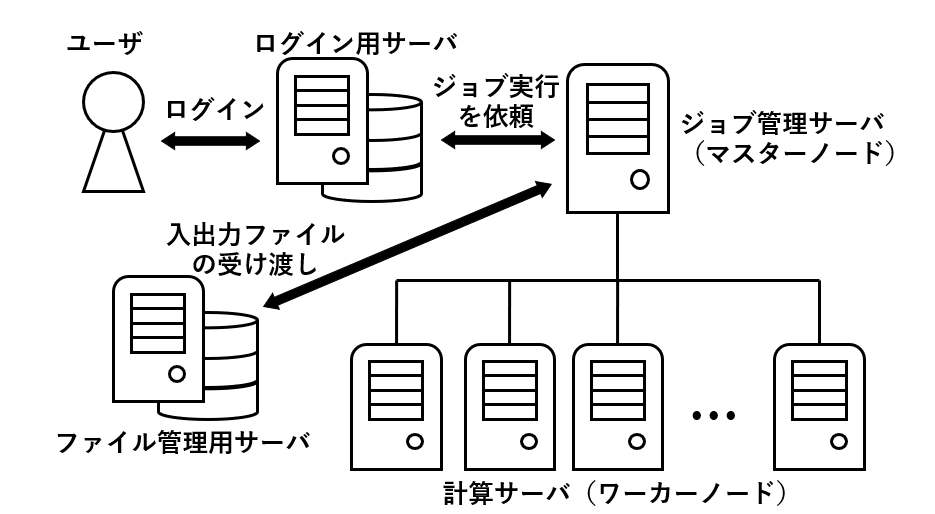
\includegraphics[width=100mm]{./fig/HPCsystem.png}
    \caption{一般的なHPCシステムの模式図}
    \label{fig4}
\end{figure}


\subsection{Open OnDemand}
代表的な関連研究として,Open OnDemand(OOD)とその機能や設計構成を紹介する\cite{cite2}\cite{cite3}.OODは米国オハイオ・スーパーコンピューティングセンターが開発したオープンソースソフトウェアであり,ウェブインタフェースを介してHPCシステムを利用できる環境を提供する.ユーザはウェブブラウザ上でHPCクラスタを簡単に操作することができ,プラグインやほかのソフトウェアのインストールや設定は不要である.また,リモートデスクトップやjupyternotebook,VSCodeなどのグラフィカルな対話的操作もウェブブラウザ上から利用することができる.OODは世界的に使われている様々なジョブスケジューラ(PBS Pro,Slurm,Grid Engine,Torque,LSFなど)に対応しているため,システム間の利用方法の差異を隠蔽している.\par
初めに,OODの機能について説明する.OODは,図\ref{dashboard}に示すダッシュボードと図\ref{homedirectory}に示すユーザのホームディレクトリを管理する画面,図\ref{activejobs}に示すジョブの状態を確認する画面,図\ref{jobcomposer}に示すジョブの管理を行う画面,図\ref{shell}に示すHPCクラスタのシェル操作を行う画面,開発者が任意の追加アプリケーションソフトウェアを導入することができるinteractiveappsから構成される.図\ref{homedirectory}に示すホームディレクトリ画面からはユーザのディレクトリを視覚的に操作することができ,ファイルやディレクトリの削除追加編集なども容易に行うことができる.図\ref{activejobs}にはジョブの状態確認を行うActive Jobs画面を示す.ユーザは投入したジョブの状態をリアルタイムで確認することができる.図\ref{jobcomposer}のJobComposerの画面では,ユーザはジョブの作成,投入,削除などをすべてこの画面から行うことができ,HPCクラスタ内のジョブの管理を行うことができる.図\ref{shell}には,シェルの操作画面を示す.ユーザは連携したHPCクラスタのシェルをウェブブラウザ上から操作することができる.このように,OODは様々な機能やアプリケーションソフトウェアと連携してHPCユーザの利用者支援を行っている.\par
続いて,OODのの設計について説明する.OODは現在多様なジョブスケジューラに対応しているが,各ジョブスケジューラへの対応はadaptersディレクトリ下に配置される.指定したジョブスケジューラに対応するために,各々でAdapterクラスのサブクラスが宣言され,内部ではジョブスケジューラに合わせてジョブの投入を行うメソッドやジョブの削除を行うメソッド,ジョブの情報を取得するメソッドが再定義されている.対応するAdaoterファイルを呼び出して参照することでOODは多様なジョブスケジューラに対応することができている.\par
以上のように,OODは視覚的かつ簡単な操作を用いてHPCシステムの利用を行うことができるというメリットを持つ.そのため,多くのコンピューティングセンターで実用化され,OODのユーザ数も年々増加しており,HPC利用環境を提供するウェブインタフェースとして多くの研究開発が行われている.\par

\begin{figure}[tb]
    \centering
    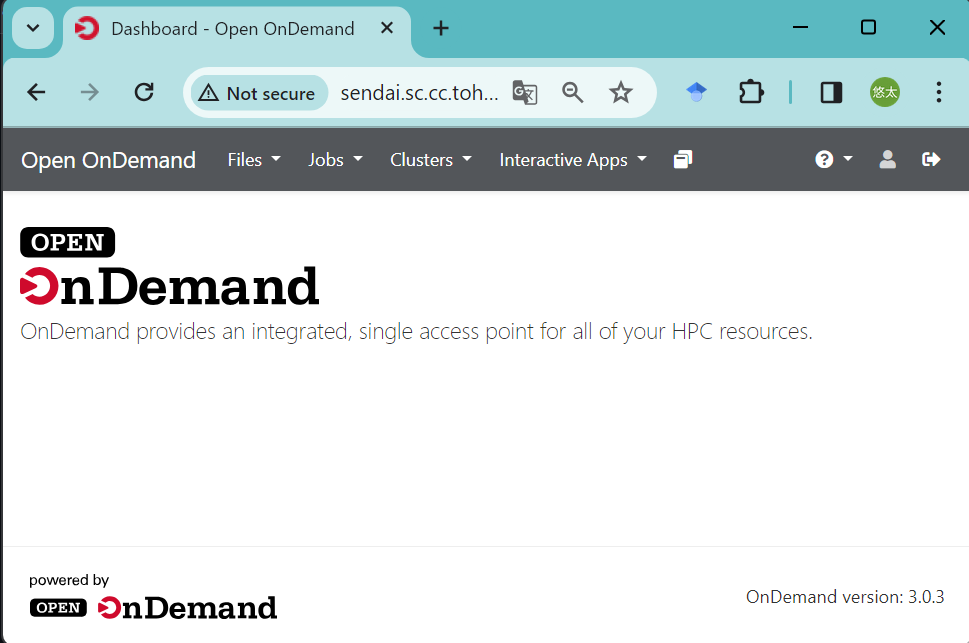
\includegraphics[width=100mm]{./fig/dashboard.png}
    \caption{ダッシュボード画面}
    \label{dashboard}
\end{figure}

\begin{figure}[tb]
    \centering
    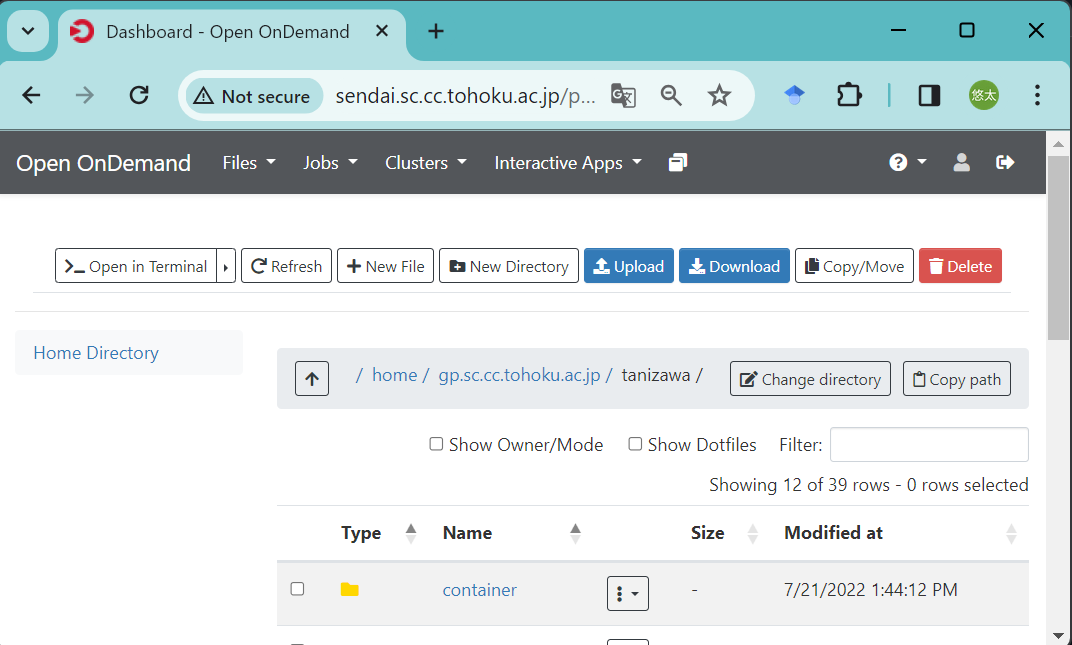
\includegraphics[width=100mm]{./fig/homedirectory.png}
    \caption{ホームディレクトリ画面}
    \label{homedirectory}
\end{figure}

\begin{figure}[tb]
    \centering
    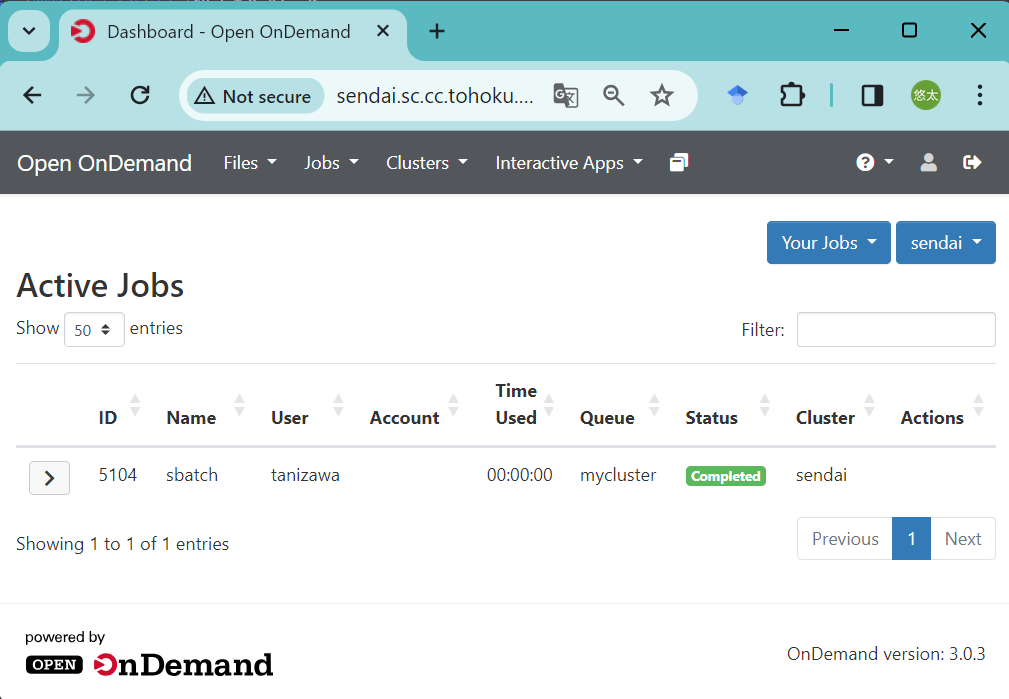
\includegraphics[width=100mm]{./fig/activejobs.png}
    \caption{ジョブ状態確認画面}
    \label{activejobs}
\end{figure}


\begin{figure}[tb]
    \centering
    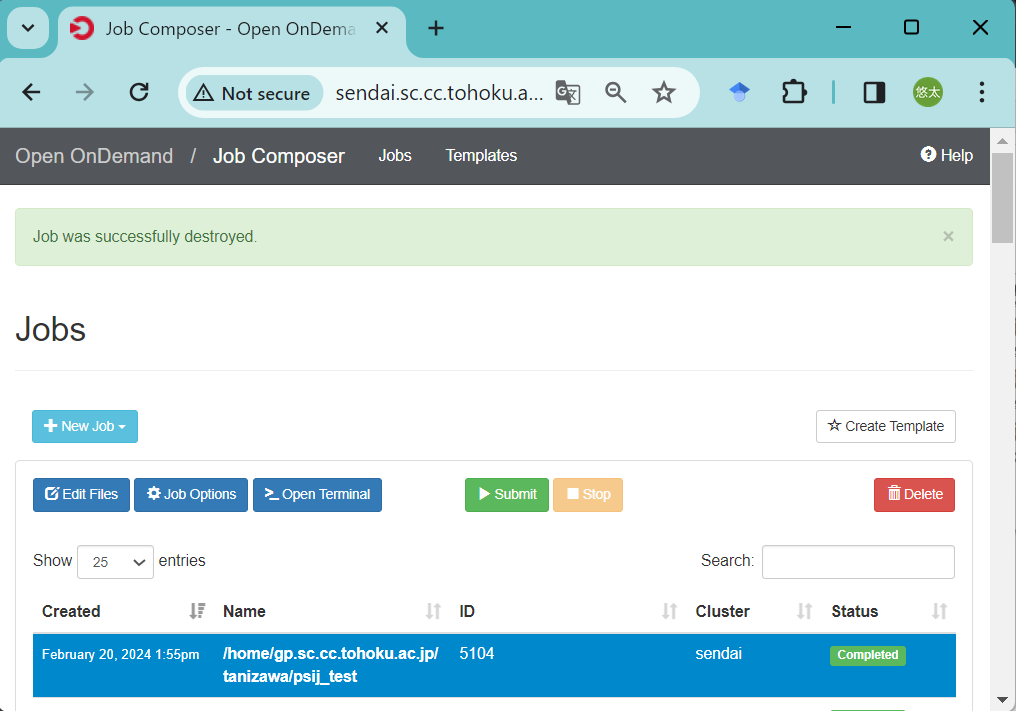
\includegraphics[width=100mm]{./fig/jobcomposer.png}
    \caption{ジョブ管理画面}
    \label{jobcomposer}
\end{figure}

\begin{figure}[tb]
    \centering
    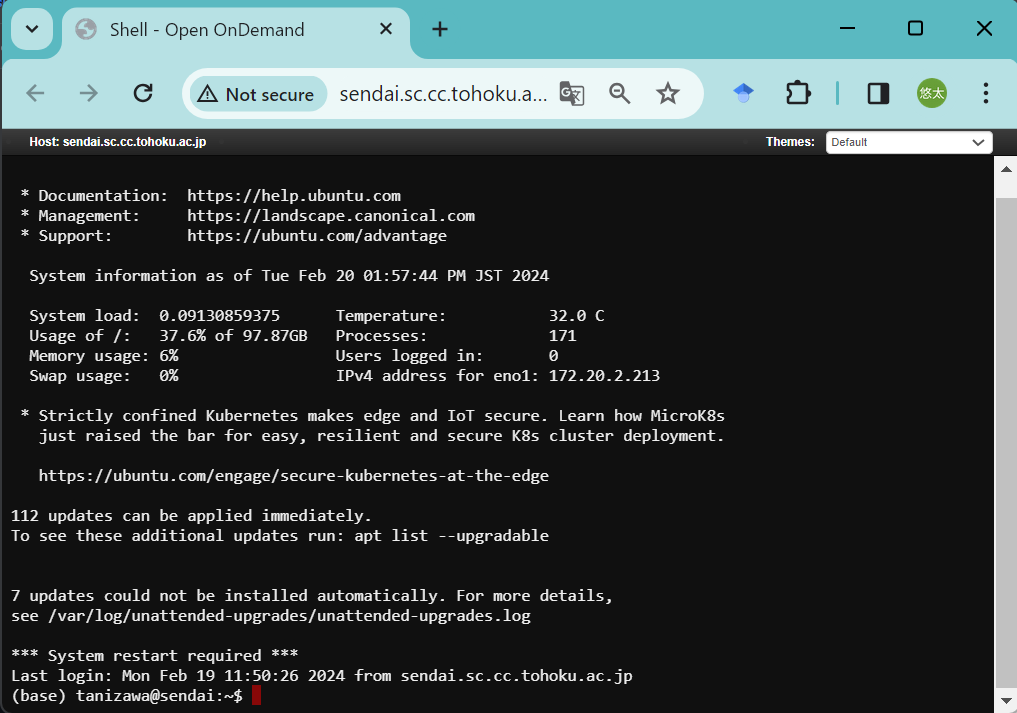
\includegraphics[width=100mm]{./fig/shell.png}
    \caption{シェル画面}
    \label{shell}
\end{figure}

\subsection{現行のウェブインタフェースにおける課題}
現行のウェブインタフェースにおける課題について説明する.OODは視覚的かつ簡単な操作を用いてHPCシステムの利用を行うことができるという大きな利点を持っている.しかし,システム設計上の課題点も考えられる.\par
国内でのウェブインタフェースの実装事例として,スーパコンピュータ富岳でのOODの実装が挙げられる.OODは汎用的なツールであるが,富岳で用いられているジョブスケジューラ(Fujitsu Technical Computing Suite, Fujitsu-TCS)に対応していなかったことから,中尾らはOODをFujitsu-TCS向けに改修した事例を報告している\cite{cite4}.Fujitsu-TCSに対応するために,新たなAdapterファイルを作成し,Fujitsu-TCS用のメソッドを再定義することによりOODはFujitsu-TCSへの対応を行うが,このような改修方法はシステムの基幹部分を直接改修しなければいけないため,慎重に作業を行う必要がある.このように,ほかにも様々なジョブスケジューラが存在し,今後も登場することを考えると,ジョブスケジューラがの種類が増えるごとにOOD本体を直接改修する方法では保守性に問題があるといえる.\par


\subsection{結言}
本章では,関連研究について述べた.はじめに一般的なHPCシステムの利用方法について説明した.基本的なHPCシステムの利用方法について説明し,基礎的な知識を解説した.その後,Open OnDemandと呼ばれるウェブインタフェースについてその機能と設計について説明した.OODを,用いることによる影響は大きく,HPCシステムのユーザに多くの利点をもたらすことができると考えられる.最後に,現行のウェブインタフェースについて,国内でのOODの実装例を参考にして課題点を述べた.ユーザに快適なHPC利用空間を提供するという利点に反して,システムの保守性が課題点として挙げられる.次章では,本章で述べた現行のウェブインタフェースにおける課題である保守性を考慮した手法を提案し,その実装を行う.\par